%!TEX root = /Users/stevenmartell/Documents/CURRENT PROJECTS/iSCAM-trunk/fba/BC-herring-2011/WRITEUP/BCHerring2011.tex
\section{Results}
	\subsection{Simulation testing}
		\subsubsection{Estimation performance with perfect information}
	
	Given perfect information about trends in relative abundance and age composition information, and a deterministic stock-recruitment relationship, \iscam\ was able to estimate 216 parameters without any substantial errors.	  Estimation performance is easily demonstrated by comparing estimates of spawning biomass and fishing mortality rates to the true values that were used to simulate the data.  As shown in Figure \ref{FigSimPlot} estimates of spawning biomass and fishing mortality rates were exactly the same as the true values. There is no measurable difference between the observed and predicted trends in the relative abundance information (Figs. \ref{FigSimPlot}cd).
	
\begin{figure}[!tbp]
	% Requires \usepackage{graphicx}
	\includegraphics[width=\textwidth]{../Figs/simPlot.pdf}\\
	\caption{True (thin line) and estimated (thick shaded line) spawning biomass (a), fishing mortality rates (b), observed and predicted relative abundance (c), and residuals between observed and predicted relative abundance (d) for the SOG herring simulation with perfect information and a deterministic stock-recruitment relationship.}\label{FigSimPlot}
\end{figure}
		
Residuals between the observed and predicted age-composition data (not shown) were also extremely small and are easily summarized by the conditional maximum likelihood estimates of the residual variance 	$\widehat{\tau}^2$ for the winter seine fishery $\widehat{\tau}^2=2.49e-03$, the seine roe fishery $\widehat{\tau}^2=1.25e-27$, and the gill net fishery  $\widehat{\tau}^2=1.24e-27$.  

This perfect fit to the data is used only to judge if the code is syntactically correct and to determine if it is capable of estimating model parameters exactly given perfect information.  In the following section, observation errors and process errors are introduced to determine bias and precision in parameter estimates.
		
		\subsubsection{Bias \& precision with observation \& process errors}

In the simulation experiments conducted with both observation error and process error included in the simulated data, there was no appreciable bias in the estimates of unfished biomass ($\ln(R_o)$) and the natural mortality rate $(\ln(M))$,  the average recruitment ($\ln(\bar{R}$) and the initial recruitment ($\ln(\dot{R})$, Figure \ref{FigSogBias}).   There was, however, a very slight upward bias in the estimate of the steepness parameter for the Beverton-Holt stock recruitment relationship.  Also, steepness was estimated with the least amount of precision.  The estimability of steepness depends on many factors including the precision of the observations, but also the history of exploitation, the true value of steepness and the natural mortality rate \citep{conn2010can}.
		
\begin{figure}[!tbp]
	% Requires \usepackage{graphicx}
	\includegraphics[width=\textwidth]{../Figs/SOGParameterBias.pdf}\\
	\caption{Estimates of precision and bias in key model parameters and MSY based reference points for 50 simulated data sets conditioned on the Strait of Georgia herring catch. The log2 ratio of estimated versus true value is plotted; values of 1 and -1 correspond to a twice or  half the true value, respectively.}\label{FigSogBias}
\end{figure}

Its not surprising to see a slight upward bias in $h$ for these simulations because the true value of natural mortality was set quite high ($M=0.45$) along with steepness ($h=0.8$).  Furthermore, the simulated exploitation history involved a strong depletion signal between the 1950s and 1960's followed by very light exploitation from 1970 onward.  On average the assumed parameter values for the simulation and the catch time series generated sufficient contrast to reliably estimate key model parameters without the use of informative priors.

The lower panel of Figure \ref{FigSogBias} shows the apparent precision and bias in the estimates of MSY based reference points.  There is a very slight upward bias in the estimate of \fmsy\ associated with the slight upward bias in steepness.  Estimates of \bmsy\ are also slightly biased in a downward direction, and MSY in a slight upward direction.  Overall, MSY is the most precisely estimated and \fmsy\ is the least precisely estimated management variable.


	\subsection{Comparison of HCAM with \iscam}
	
	Based on the description of the priors and model setup in Section \ref{secMethodsHCAM} on page \pageref{secMethodsHCAM}, a comparison of the spawning stock biomass between \iscam\ and HCAM were very similar (Figure \ref{fig1_HCAM_ctrl}a) for the Strait of Georgia stock.  Between 1951 and 1969 the absolute difference in spawning biomass is minimal and post 1970 estimates of spawning biomass are slightly higher for the HCAM model. The only real difference between the two models during this period is a differences in the assumptions about the error structure for the age-composition data.
	
	Estimates of spawning depletion are based on the post fishery spawning biomass relative to the estimated unfished spawning biomass (Figure \ref{fig1_HCAM_ctrl}b).  The three coloured zones demarcate the critical zone, cautious zone, and healthy zones which are defined by 0.4\bmsy\ and 0.8\bmsy, respectively.
	
Maximum likelihood estimates of key model parameters for both \iscam\ and HCAM are summarized in Table \ref{TableHCAMcompare}.    The \iscam\ model tends to have a lower estimate of $B_o$ in comparison to the HCAM model and a  higher value of steepness ($h$).  These two parameters are usually negatively correlated and it is expected that if $B_o$ was higher in one model in comparison to the other, then $h$ would normally be lower to compensate.  Information to estimate $B_o$ and $h$ come from the apparent stock-recruitment data and the structural form of the stock recruitment relationship.  In \iscam\ annual recruitment is freely estimated and the residuals are based on the Beverton-Holt stock recruitment model and the estimates of spawning stock biomass.  Similarly, in HCAM recruitment is a function of the spawning stock biomass and the Beverton-Holt model and the annual deviations are estimated and assumed to be normally distributed random variables.



\begin{table}[htdp]
\caption{A comparison of key parameters from \iscam\ and the HCAM model}
\begin{center}
\begin{tabular}{lll}
\hline
Parameter & \iscam\ & HCAM \\ \hline
Unfished spawning biomass ($B_o$ 1000 t) & 114.492 & 190.817\\
Steepness ($h$) & 0.786  &  0.683\\
Average natural mortality rate & 0.535 &  0.334\\
Survey $q$ for period 1 & 1.101  & 1.1105\\
\hline
\end{tabular}
\end{center}
\label{TableHCAMcompare}
\end{table}%

%% Revisions required below with updates.

Average natural mortality rate is higher in the \iscam\ model (Table \ref{TableHCAMcompare}), and the survey $q$ for the pre-1988 spawn survey data is nearly identical in the two models (Figure \ref{fig1_HCAM_ctrl}f).  The more contemporary survey data were both forced to scale with $q=1.0$.  There is some pattern in the residuals for the overall fits to the survey data (Figure \ref{fig1_HCAM_ctrl}f), the model fails to predict the large increases in abundance in the late 1970s and early 2000s and the recent sharp decline in the mid 2000s.  The assumed standard deviation for the survey errors was 0.35 and 0.3 for the pre and post 1988 survey data, the standard deviation of the residual errors in Figure \ref{fig1_HCAM_ctrl}d is 0.335 and 0.334, respectively.
	
\begin{figure}[!tbp]
	% Requires \usepackage{graphicx}
	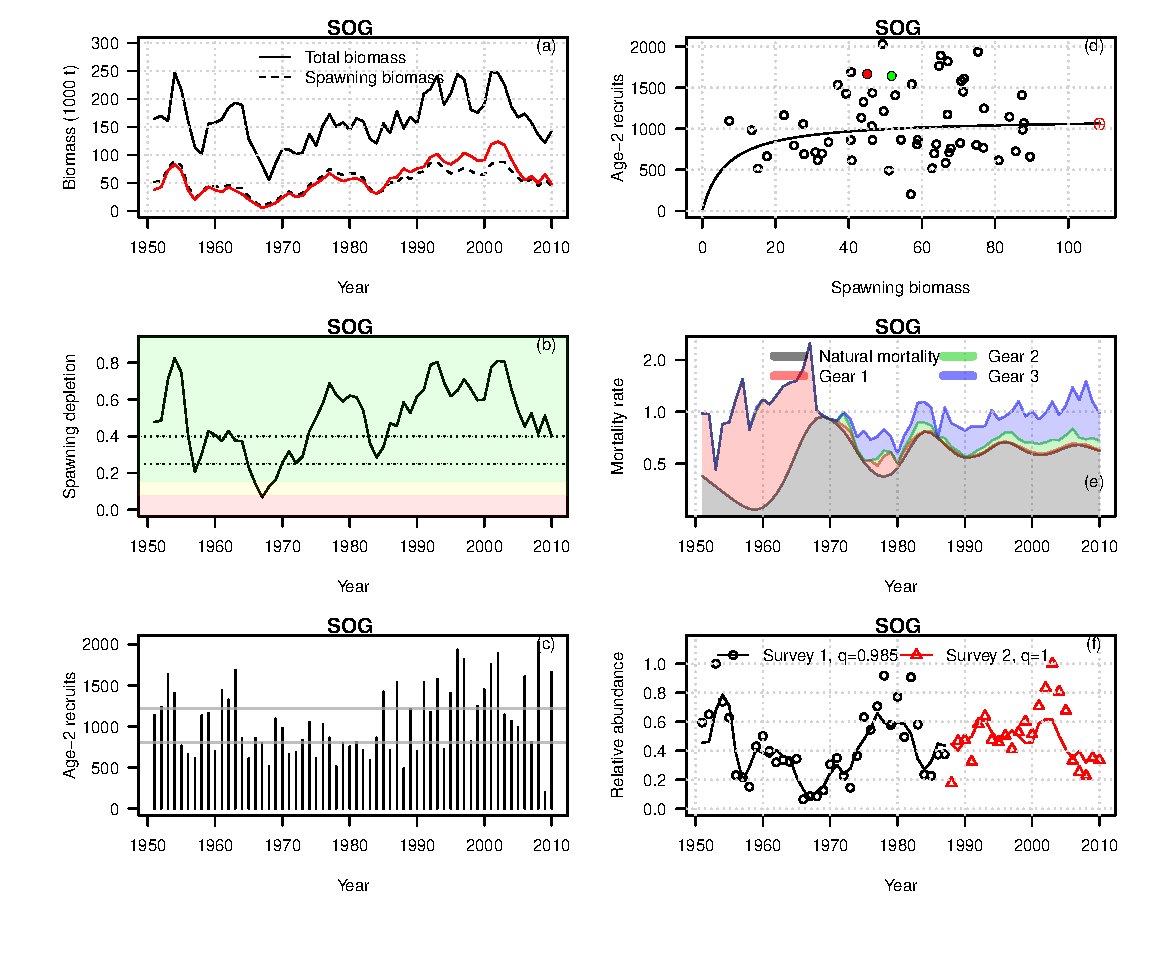
\includegraphics[width=\textwidth]{../Figs/iscam_fig_HCAM_SOG_MLE.pdf}\\
	\caption{Maximum likelihood estimates of pre-fishery biomass (defined as the numbers-at-age times the mean weight-at-age at the start of the year) and post fishery spawning biomass in the Strait of Georgia (a), spawning biomass depletion (b), age-2 recruits (c), stock-recruitment relationship and unfished reference points (d), components of total mortality (log-scale, e), and observed (points) and predicted (lines) spawn survey data (f).  These results are based on trying to configure the \iscam\ model as similar as possible to the previous HCAM assessment; the red line in panel (a) is the MLE estimate of spawning biomass from HCAM.}\label{fig1_HCAM_ctrl}
\end{figure}


Estimates of the components of total mortality for the comparison with the HCAM model are shown in Figure \ref{fig1_HCAM_ctrl}e.  The fishing mortality rates for each gear represent the average fishing mortality rate over all age-classes, and the natural mortality rate is assumed to be age-independent.  During the 1950s through to 1968, fishing mortality rates for Pacific herring in the Strait of Georgia were extremely high; this period was almost exclusively a purse-seine fishery where fish were taken for fishmeal.  After the fishery reopened in the early 1970s fishing mortality rates were greatly reduced and targeted the spawning component of the stock as the market was for herring roe. 

Estimates of natural mortality are based on a random walk process, initially starting at a value of 0.401 in 1951 and declining to a very low value of 0.217 in 1959, then increasing to a maximum of 0.915 in 1969 (Figure \ref{fig1_HCAM_ctrl}e).  Information to estimate natural mortality rates comes from the age-composition data, and assumptions about selectivity in the fishery.  In this comparison, the \iscam\ model assumes selectivity is invariant for the purse seine gears and is a function of weight-at-age for the gill net gear. Much of the residual variation in the age-composition is explained by variation in $M$ and variation in age-2 recruits (see Figures \ref{fig1_HCAM_ctrl}c \& d for and age-2 recruitment and stock recruitment relationship).  The HCAM model has a very similar trend in the estimates of natural mortality but the variability is much less than that of the \iscam\ assessment.  This is almost certainly due to the differences in the assumptions about the error structure in the age-composition data (or relative weights associated with the age-composition).




\begin{figure}[!tbp]
	% Requires \usepackage{graphicx}
	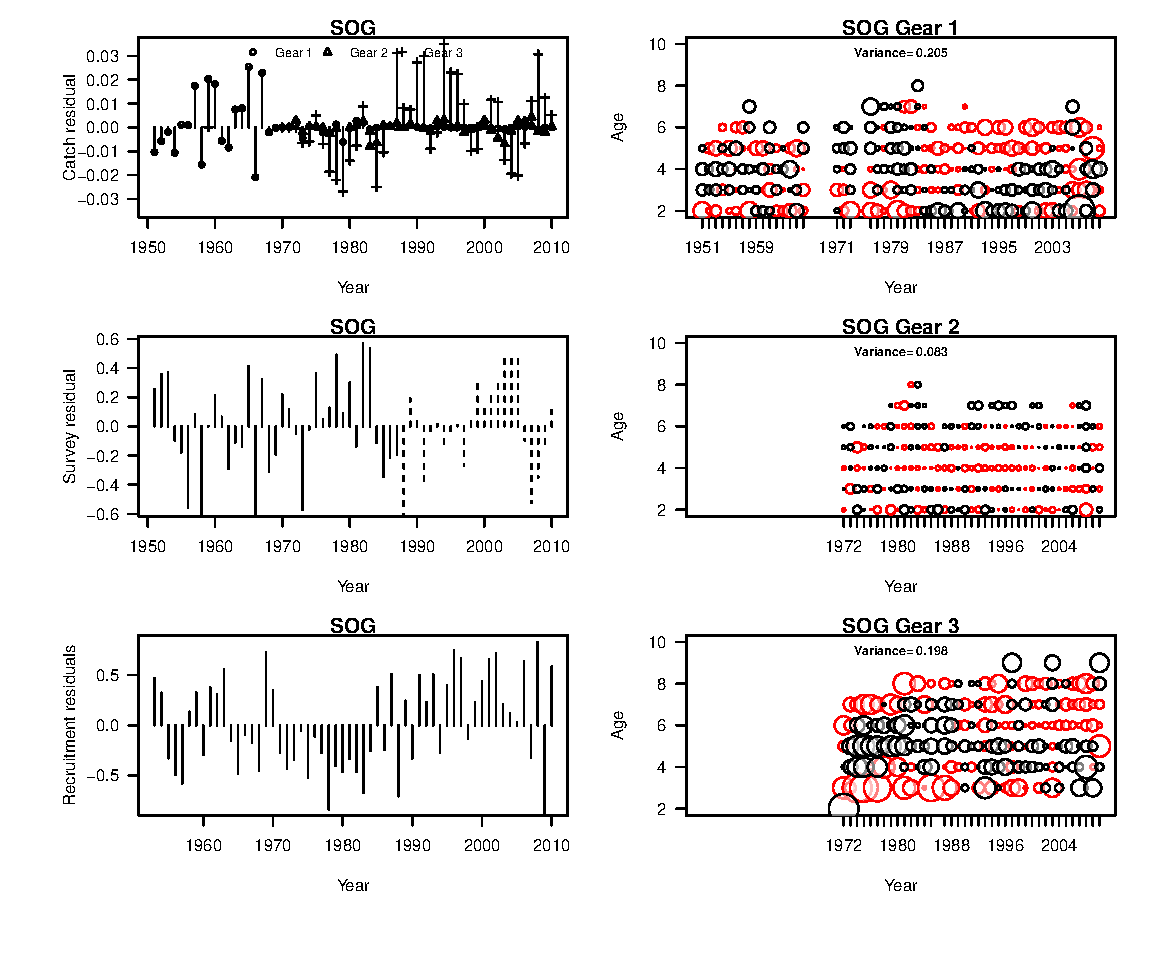
\includegraphics[width=\textwidth]{../FIGS/iscam_fig_HCAM_SOG_RES.pdf}\\
	\caption{From top to bottom in the left column: the log residuals between observed and predicted catch for each gear, the residuals between the observed and predicted spawn survey index, and the annual deviations between age-2 recruitment and that predicted by the Beverton-Holt model and the estimated spawning stock biomass. Right column: residual patterns in the age-composition data (observed - predicted, where black is a positive residual) for each of the three commercial gears in the Strait of Georgia.}\label{fig_HCAM_SOG_RES}
\end{figure}

There is good correspondence between the observed and predicted catch, however, the residual patterns does not appear to be iid for each of the fleets (Fig. \ref{fig_HCAM_SOG_RES}).  Recall that the fit to the catch data is largely determined by an assumed variance for the observation errors in the reported catch ($\sigma_C^2=0.005$).   

The fit to the spawn survey data in Strait of Georgia is nearly iid for the 1951:1987 time period.  There is some pattern in the residuals post 1988 that appears to be in contradiction with other information (i.e., age-composition data and structural assumptions about selectivity) (Fig. \ref{fig_HCAM_SOG_RES}).  The pattern in the recruitment residuals for the Strait of Georgia suggest periods of below average-recruitment in the 1970s and early 1980s and above average recruitment starting in the early 1990s.


Fits to the age-composition data for the purse seine-roe fishery were best in comparison to the winter seine and gillnet fisheries.   The conditional maximum likelihood estimates of the variance of the age-composition data are 0.205, 0.083, and 0.198 for the winter purse seine, seine-roe, and gill net fisheries, respectively.The smaller the standard deviation, the better correspondence between the observed and predicted age-composition data.  Also the pattern of residuals does indicate some model mis-specification (e.g., the gillnet fishery in the Strait of Georgia).



%\begin{figure}[!tbp]
%	% Requires \usepackage{graphicx}
%	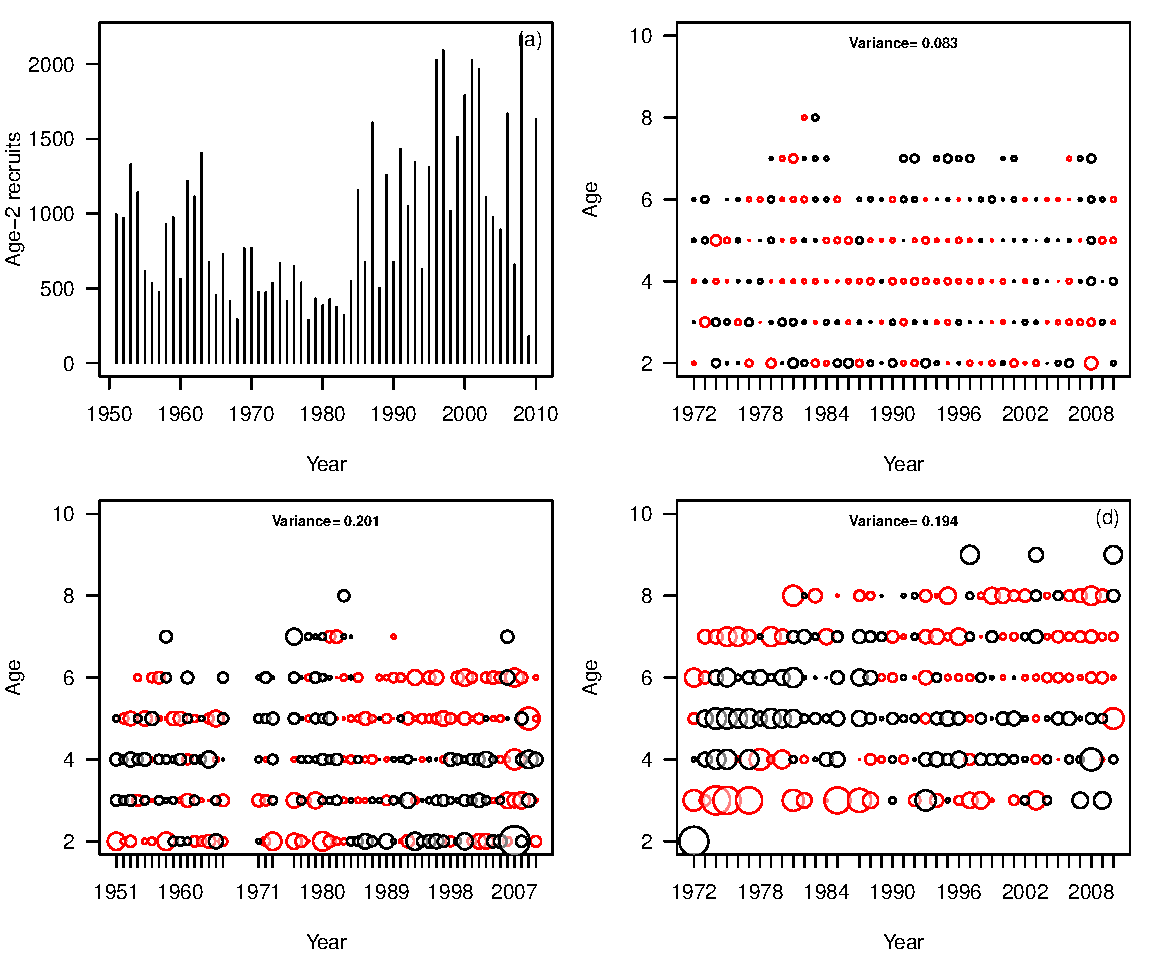
\includegraphics[width=\textwidth]{../Figs/fig3_HCAM_ctrl.pdf}\\
%	\caption{Estimates of age-2 recruits (a) and the residuals (observed-predicted, positive shown in black)  in the age-composition data for the winter purse seine fishery (lower left), seine-roe fishery (upper right) and gill net fishery (lower right). The area of each circle is proportional to the residual error, and zeros are not shown. Note that observed age-proportions less than 2\% were pooled into the adjacent (younger) age class and the conditional maximum likelihood estimates of the variance is displayed on the top of each panel.}\label{fig3_HCAM_ctrl}
%\end{figure}

%\begin{figure}[!tbp]
%	% Requires \usepackage{graphicx}
%	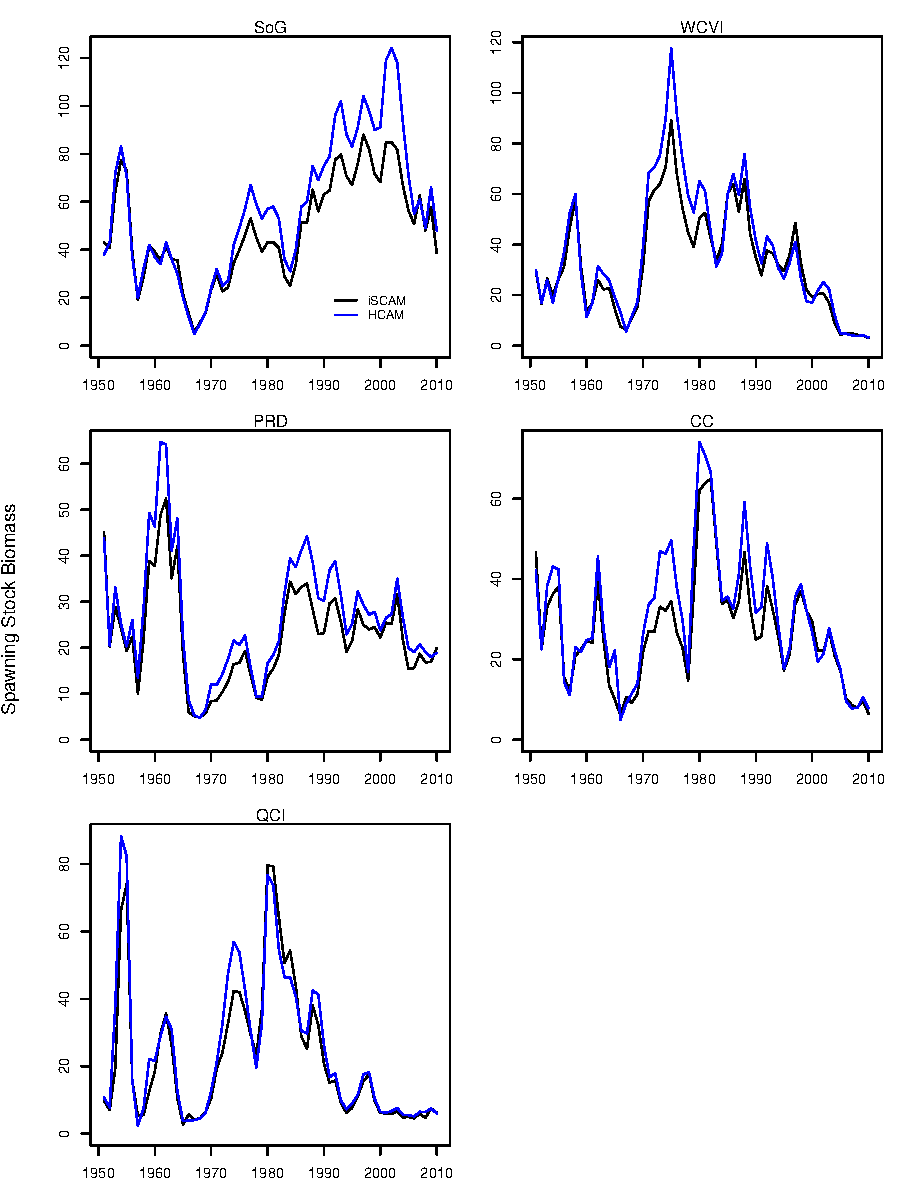
\includegraphics[width=0.9\textwidth]{../Figs/figHCAMvsiSCAM.pdf}\\
%	\caption{A comparison of estimated spawning stock biomass between HCAM and \iscam\ for the five major stock assessment regions.}\label{figHCAMvsiSCAM}
%\end{figure}


	\subsection{Alternative assumptions about catchability, mortality \& selectivity}
	
	Here we briefly explore the differences between relaxing the informative prior on catchability for the survey, reducing the number of natural mortality parameters being estimated and exploring alternative selectivity options to try and reduce the residual pattern in the gillnet fishery age-composition data.  For the comparisons, we only examine the maximum likelihood fits to the data and the overall objective function value.
	
The following table presents a few summary statistics in the following section for easier comparison.

\begin{table}[htdp]
\caption{Summary statistics for alternative structural assumptions about the Strait of Georgia herring assessment from 1951 to 2010.  Definitions are No. is the number of estimated parameters, $f$ the objective function value, $B_o$ unfished spawning biomass, $h$ steepness, $\bar{M}$ is the average natural mortality rate, \bmsy the biomass at maximum sustainable yield, $q$ survey scalers for pre and post 1988.}\label{Table:HCAM_stats}
\begin{center}
\begin{tabular}{lllllllll}
\hline
Model & No. & $f$ & $B_o$& $h$ & $\bar{M}$ & \bmsy & $q_1$ & $q_2$\\
\hline
Fixed $q$ & 279 & -1165.77 & 114.93 & 0.786 & 0.53 & 23.114 & 1.01 & 1.0\\ 
Prior $q$ & 279 & -1161.49 & 116.98 & 0.766 & 0.58 & 24.370 & 0.988 & 0.878\\
Fixed $M$ & 219 & -1051.92 & 126.59 & 0.706 & 0.68 & 28.510 & 0.681 & 0.795\\
Gill net Selectivity & 279 & -1196.06 & 121.65 & 0.76 & 0.655 & 25.27 & 0.817 & 0.795\\ 
\hline
\end{tabular}
\end{center}
\end{table}%


	
		\subsubsection{Impacts of informative priors on $q$'s}
The implication of relaxing the informative prior on $q$ for the contemporary spawn survey data was examined by using a less informative prior for the spawn survey $q$. The results shown in Fig. \ref{fig:qFix_qPrior} is a comparison of the HCAM parameterized version of the model as shown in previous sections with a version where the prior on $\ln(q)$ was assumed normal ($\mu=0, \sigma = 0.274$) for both the contemporary and surface survey data.
\begin{figure}[!tbp]
	% Requires \usepackage{graphicx}
	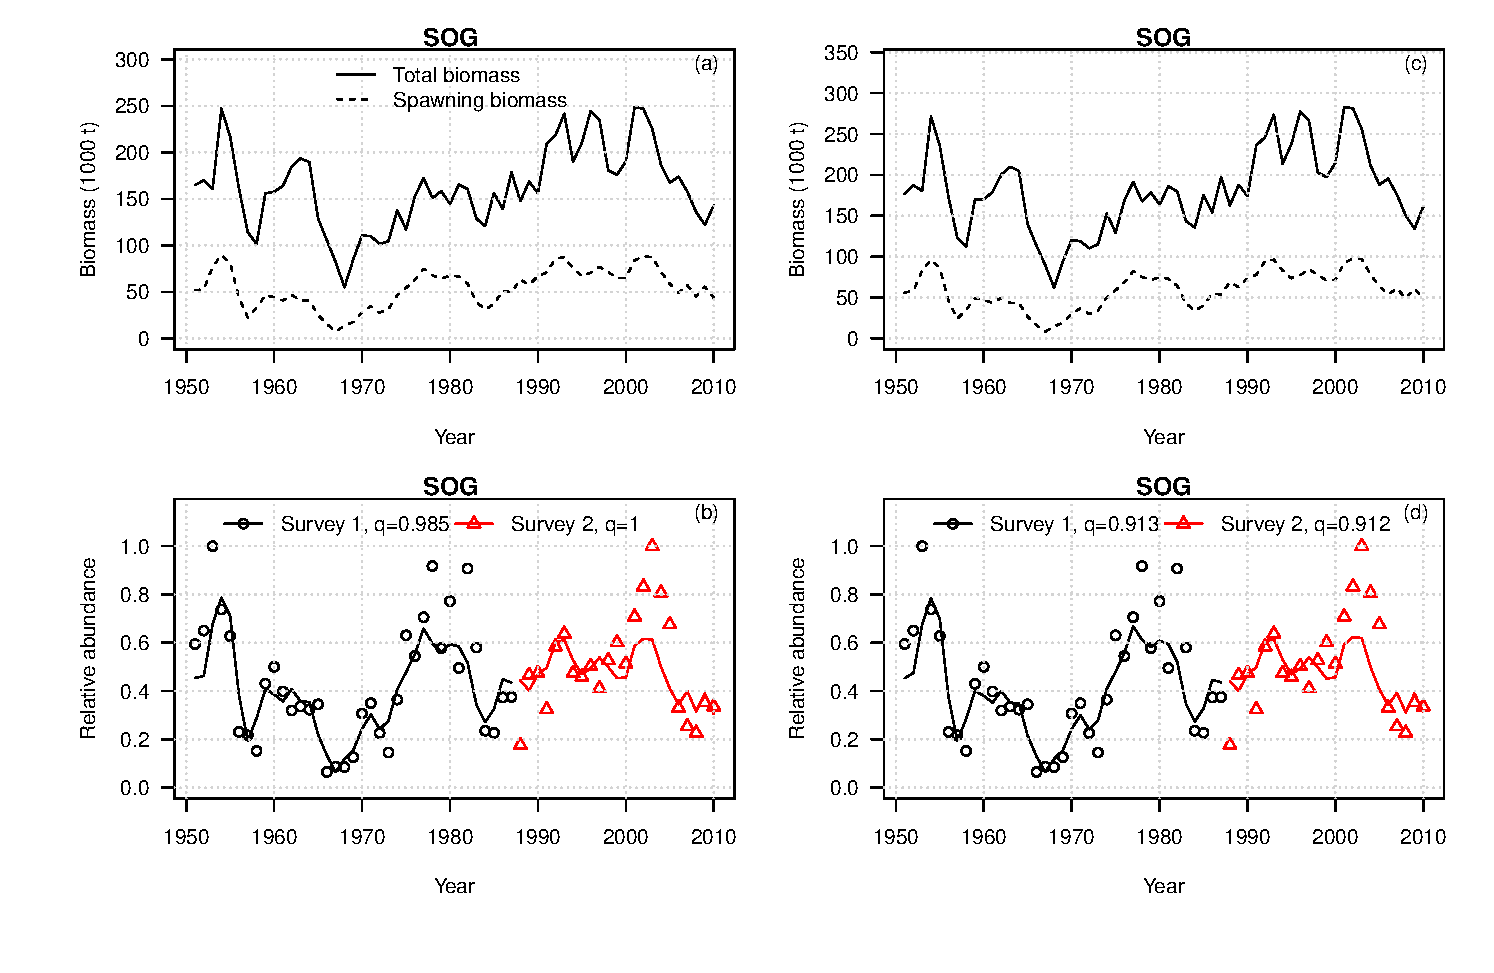
\includegraphics[width=\textwidth]{../FIGS/iscam_fig_HCAM_qFix_qPrior.pdf}\\
	\caption{A comparison of the estimated biomass and spawning biomass and fits to the survey data when q is either fixed at 1 for Survey 2, or  estimated using an informative prior with an expected mean of 0 and a log standard deviation of 0.274.}\label{fig:qFix_qPrior}
\end{figure}

The net result of relaxing this prior on $q$ is a slight increase in the global scaling (the spawn biomass increases by roughly 12\%) in comparison to the fixed $q=1$ scenario.  There is no appreciable difference in the overall fits to the data (see objective function value in Table \ref{Table:HCAM_stats}.
		
		\subsubsection{Implications of variable natural mortality rate $M_t$}
	In this next scenario we use the same prior for $\ln(q)$ but do not allow natural mortality rates to vary over time (i.e., fixed $M$).  The natural mortality rate and $q$ are confounded so it does not make sense to fix $q$ and estimate $M$ because the corresponding estimate of $M$ would simply be conditional on the assumed value of $q$.
	
\begin{figure}[!tbp]
	% Requires \usepackage{graphicx}
	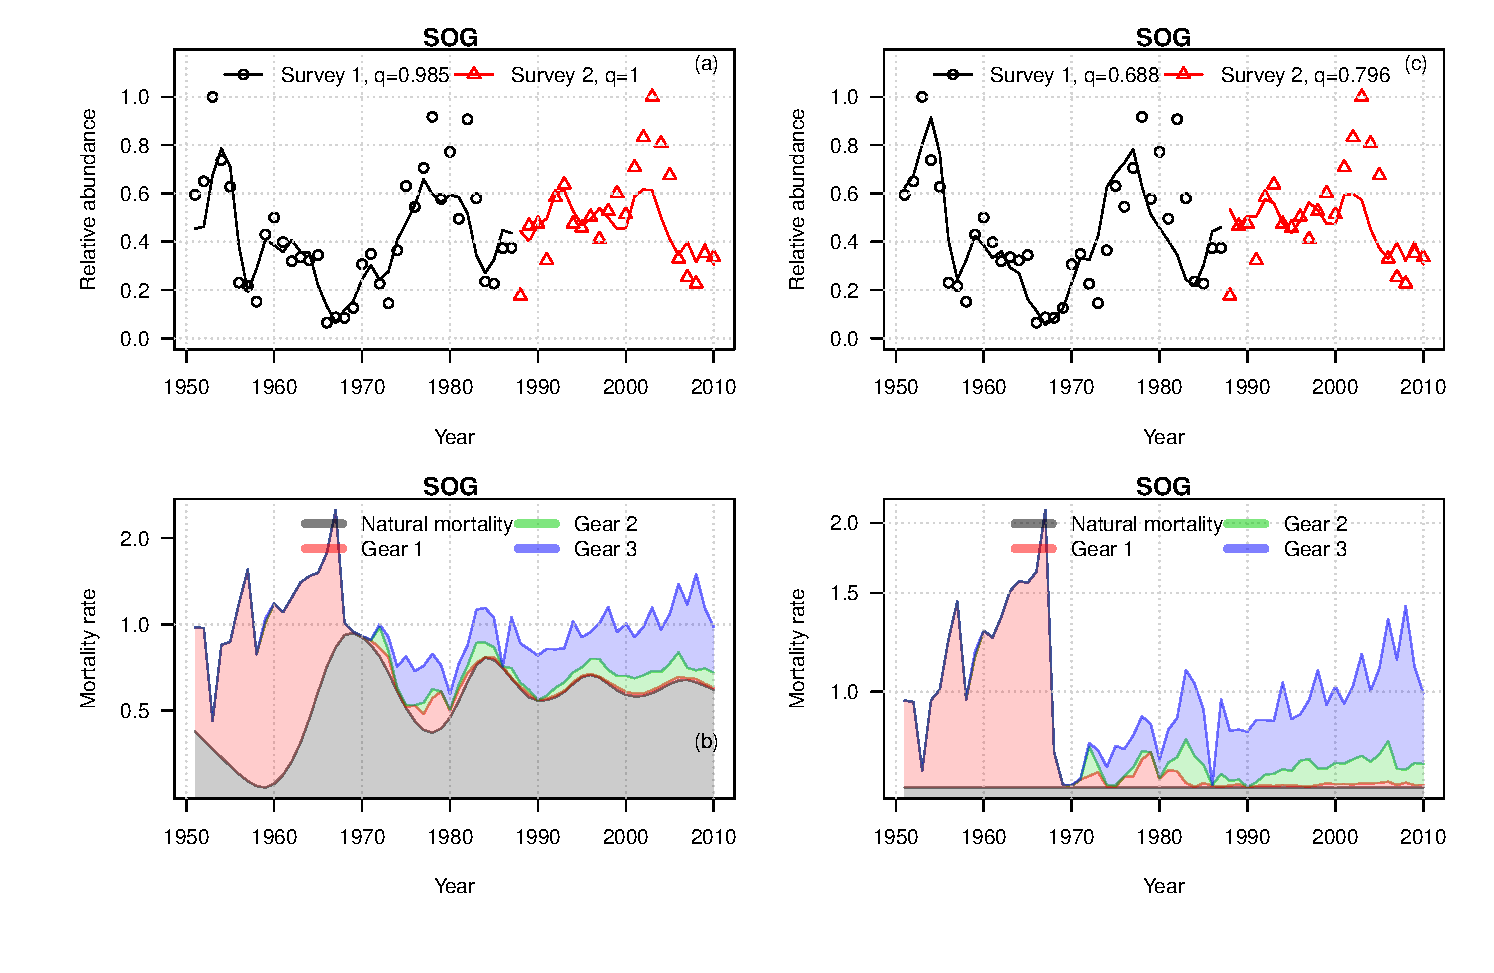
\includegraphics[width=\textwidth]{../FIGS/iscam_fig_HCAM_qFix_Mfix.pdf}\\
	\caption{A comparison of fits to the survey data and estimated components of average mortality by year when $M$ is allowed to vary via a random walk process or is estimated and assumed time invariant. }\label{fig:qFix_Mfix}
\end{figure}
		
In the case where $M$ is assumed to be time invariant, estimates of average $M$ over the entire time series does increase slightly as well as the overall scaling of population size (Table \ref{Table:HCAM_stats}).  There are 60 fewer estimated parameters in this case but the overall fit to the data is slightly degraded (Fig \ref{fig:qFix_Mfix}).
		
		\subsubsection{Implications of variable selectivity in directed fisheries}

Finally, we also explored the option of treating the gill net selectivity as time invariant and estimated two parameters that describe age-specific selectivity using a logistic curve.	In this case we also allowed for a random walk  process in natural mortality rates so the total number of estimated parameters remains the same. 

\begin{figure}[!tbp]
	% Requires \usepackage{graphicx}
	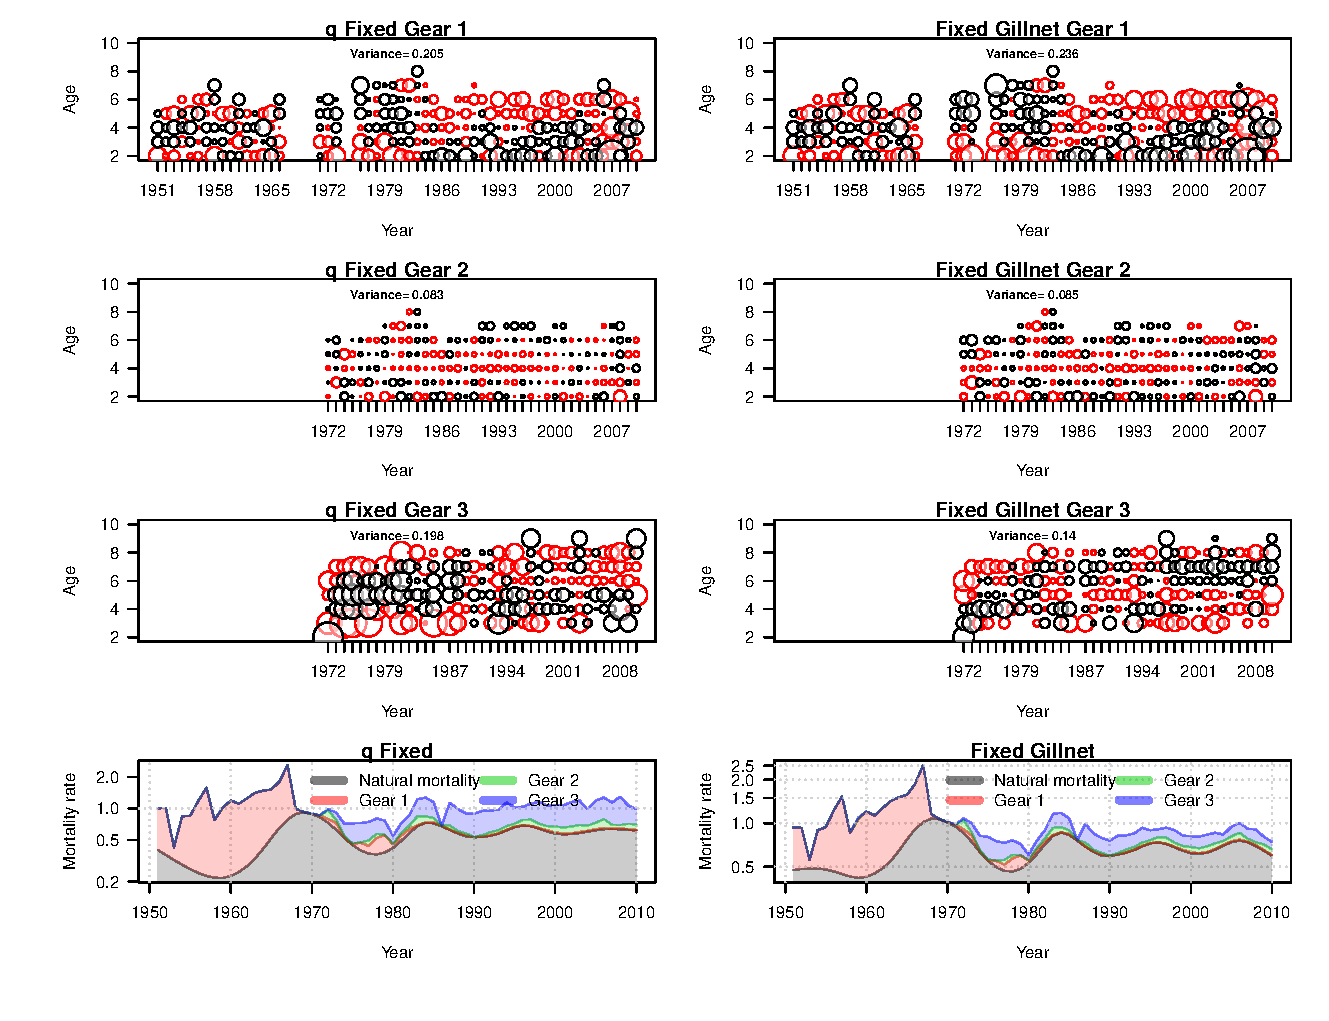
\includegraphics[width=\textwidth]{../FIGS/iscam_fig_HCAM_Ares_qFix_GillFix.pdf}\\
	\caption{Residuals in the age-composition data when gill net selectivity is a function of mean weight-at-age (left column) and or is a logistic function of age and time invariant (right colum).}\label{fig:qFix_GillFix}
\end{figure}

Slightly better fits were obtained to the gill net fishery age-composition data with a constant selectivity, and the residual pattern also appears to improve under the assumption of constant selectivity (Fig. \ref{fig:qFix_GillFix}).  There was also a slight degradation to the age composition data in the winter purse seine fishery (Gear 1), but residual patterns were nearly identical in both the seine fisheries (Fig. \ref{fig:qFix_GillFix}).  The same number of model parameters were estimated and there was a slight improvement in the overall objective function with constant selectivity (Table \ref{Table:HCAM_stats}).  However, there is much more variability in the estimates of natural mortality rates when the gill net selectivity is assumed constant.


	
%	\subsection{Separating test fishery data from the purse seine roe fishery data}
	
	
	\subsection{Preliminary assessments for all other areas}
	For the five major stock assessment regions there was very good correspondence between the estimated spawning stock biomass between the HCAM and new \iscam\  models (Fig. \ref{fig:iSCAMvsHCAM}). The control file used for each of the assessment regions was the same as that used for the Strait of Georgia.  No additional changes were required (i.e., each SAR had the same initial starting parameter values etc.).

\begin{figure}[htbp]
	\centering
		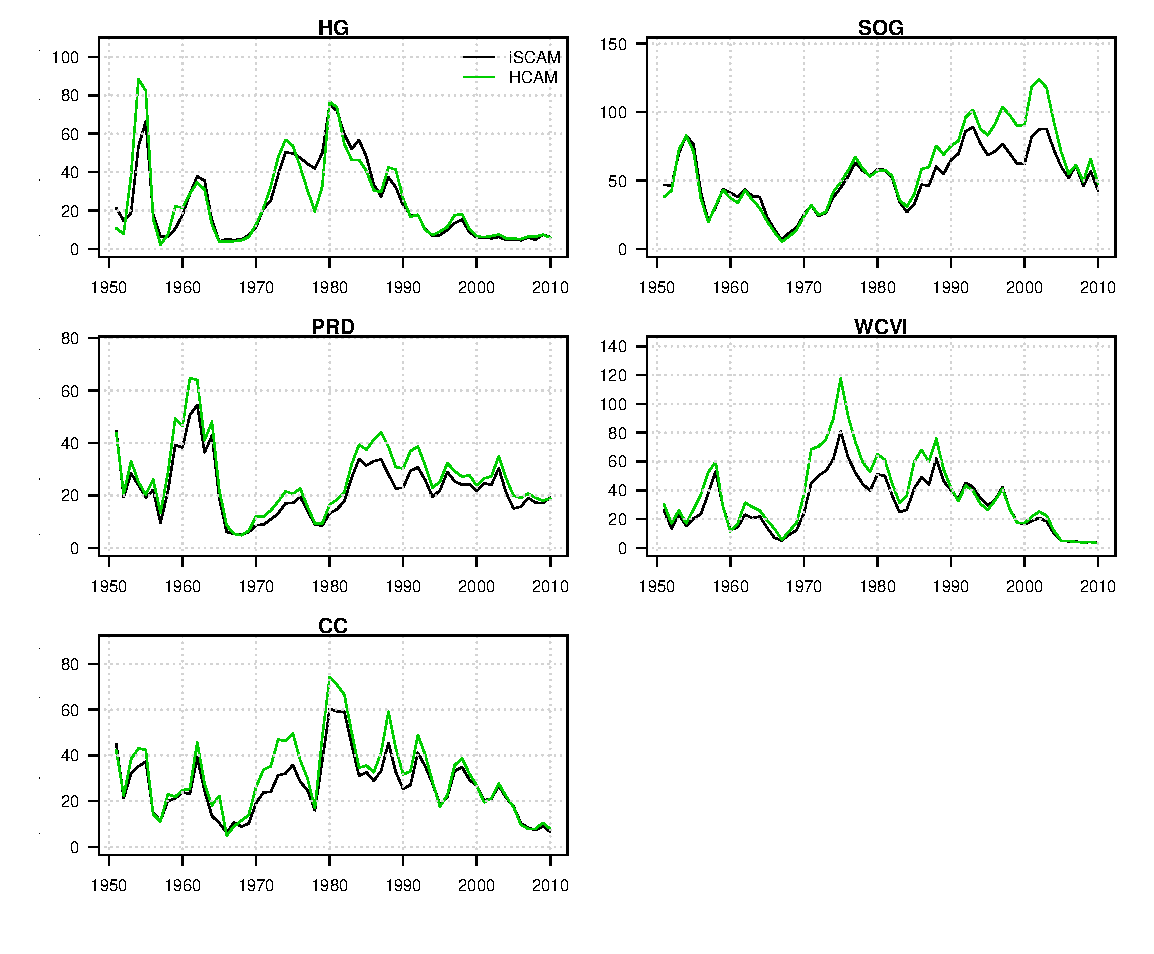
\includegraphics[width=\textwidth]{../Figs/iscam_fig_SBt_iSCAMvsHCAM.pdf}\\
	\caption{A comparison of estimated spawning stock biomass between HCAM and \iscam\ for the five major stock assessment regions using data from 1951 to 2010 and setting up \iscam\ similar to HCAM.}
	\label{fig:iSCAMvsHCAM}
\end{figure}

\clearpage
%%%%%%%%%%%%%%%%%%%%%%%%%%%%%%%%%%%%%%%%%%%%%%%%%%%%%%%%%%%%%
%% END 														 %%
%%%%%%%%%%%%%%%%%%%%%%%%%%%%%%%%%%%%%%%%%%%%%%%%%%%%%%%%%%%%%
